% Options for packages loaded elsewhere
\PassOptionsToPackage{unicode}{hyperref}
\PassOptionsToPackage{hyphens}{url}
\PassOptionsToPackage{dvipsnames,svgnames,x11names}{xcolor}
%
\documentclass[
  letterpaper,
  DIV=11,
  numbers=noendperiod,
  titlepage=false]{scrreprt}

\usepackage{amsmath,amssymb}
\usepackage{iftex}
\ifPDFTeX
  \usepackage[T1]{fontenc}
  \usepackage[utf8]{inputenc}
  \usepackage{textcomp} % provide euro and other symbols
\else % if luatex or xetex
  \usepackage{unicode-math}
  \defaultfontfeatures{Scale=MatchLowercase}
  \defaultfontfeatures[\rmfamily]{Ligatures=TeX,Scale=1}
\fi
\usepackage{lmodern}
\ifPDFTeX\else  
    % xetex/luatex font selection
\fi
% Use upquote if available, for straight quotes in verbatim environments
\IfFileExists{upquote.sty}{\usepackage{upquote}}{}
\IfFileExists{microtype.sty}{% use microtype if available
  \usepackage[]{microtype}
  \UseMicrotypeSet[protrusion]{basicmath} % disable protrusion for tt fonts
}{}
\makeatletter
\@ifundefined{KOMAClassName}{% if non-KOMA class
  \IfFileExists{parskip.sty}{%
    \usepackage{parskip}
  }{% else
    \setlength{\parindent}{0pt}
    \setlength{\parskip}{6pt plus 2pt minus 1pt}}
}{% if KOMA class
  \KOMAoptions{parskip=half}}
\makeatother
\usepackage{xcolor}
\setlength{\emergencystretch}{3em} % prevent overfull lines
\setcounter{secnumdepth}{-\maxdimen} % remove section numbering
% Make \paragraph and \subparagraph free-standing
\ifx\paragraph\undefined\else
  \let\oldparagraph\paragraph
  \renewcommand{\paragraph}[1]{\oldparagraph{#1}\mbox{}}
\fi
\ifx\subparagraph\undefined\else
  \let\oldsubparagraph\subparagraph
  \renewcommand{\subparagraph}[1]{\oldsubparagraph{#1}\mbox{}}
\fi


\providecommand{\tightlist}{%
  \setlength{\itemsep}{0pt}\setlength{\parskip}{0pt}}\usepackage{longtable,booktabs,array}
\usepackage{calc} % for calculating minipage widths
% Correct order of tables after \paragraph or \subparagraph
\usepackage{etoolbox}
\makeatletter
\patchcmd\longtable{\par}{\if@noskipsec\mbox{}\fi\par}{}{}
\makeatother
% Allow footnotes in longtable head/foot
\IfFileExists{footnotehyper.sty}{\usepackage{footnotehyper}}{\usepackage{footnote}}
\makesavenoteenv{longtable}
\usepackage{graphicx}
\makeatletter
\def\maxwidth{\ifdim\Gin@nat@width>\linewidth\linewidth\else\Gin@nat@width\fi}
\def\maxheight{\ifdim\Gin@nat@height>\textheight\textheight\else\Gin@nat@height\fi}
\makeatother
% Scale images if necessary, so that they will not overflow the page
% margins by default, and it is still possible to overwrite the defaults
% using explicit options in \includegraphics[width, height, ...]{}
\setkeys{Gin}{width=\maxwidth,height=\maxheight,keepaspectratio}
% Set default figure placement to htbp
\makeatletter
\def\fps@figure{htbp}
\makeatother

% load packages
\usepackage{geometry}
\usepackage{xcolor}
\usepackage{eso-pic}
\usepackage{fancyhdr}
\usepackage{sectsty}
\usepackage{fontspec}
\usepackage{titlesec}

%% Set page size with a wider right margin
\geometry{a4paper, total={170mm,257mm}, left=20mm, top=20mm, bottom=20mm, right=50mm}

%% Let's define some colours
\definecolor{light}{HTML}{FFD700}
\definecolor{highlight}{HTML}{800080}
\definecolor{dark}{HTML}{330033}

%% Let's add the border on the right hand side 
\AddToShipoutPicture{% 
    \AtPageLowerLeft{% 
        \put(\LenToUnit{\dimexpr\paperwidth-3cm},0){% 
            \color{light}\rule{3cm}{\LenToUnit\paperheight}%
          }%
     }%
     % logo
    \AtPageLowerLeft{% start the bar at the bottom right of the page
        \put(\LenToUnit{\dimexpr\paperwidth-2.25cm},27.2cm){% move it to the top right
            \color{light}
\includegraphics[width=1.5cm]{_extensions/nrennie/PrettyPDF/rosemary.png}
          }%
     }%
}

%% Style the page number
\fancypagestyle{mystyle}{
  \fancyhf{}
  \renewcommand\headrulewidth{0pt}
  \fancyfoot[R]{\thepage}
  \fancyfootoffset{3.5cm}
}
\setlength{\footskip}{20pt}

%% style the chapter/section fonts
\chapterfont{\color{dark}\fontsize{20}{16.8}\selectfont}
\sectionfont{\color{dark}\fontsize{20}{16.8}\selectfont}
\subsectionfont{\color{dark}\fontsize{14}{16.8}\selectfont}
\titleformat{\subsection}
  {\sffamily\Large\bfseries}{\thesection}{1em}{}[{\titlerule[0.8pt]}]
  
% left align title
\makeatletter
\renewcommand{\maketitle}{\bgroup\setlength{\parindent}{0pt}
\begin{flushleft}
  {\sffamily\huge\textbf{\MakeUppercase{\@title}}} \vspace{0.3cm} \newline
  {\Large {\@subtitle}} \newline
  \@author
\end{flushleft}\egroup
}
\makeatother

% Redefine \tableofcontents to not clear the page
\let\oldtableofcontents\tableofcontents
\renewcommand{\tableofcontents}{
  \begingroup
  \let\clearpage\relax
  \let\cleardoublepage\relax
  \oldtableofcontents
  \endgroup
}

%% Use some custom fonts
\setsansfont{Ubuntu}[
    Path=_extensions/nrennie/PrettyPDF/Ubuntu/,
    Scale=0.9,
    Extension = .ttf,
    UprightFont=*-Regular,
    BoldFont=*-Bold,
    ItalicFont=*-Italic,
    ]

\setmainfont{Ubuntu}[
    Path=_extensions/nrennie/PrettyPDF/Ubuntu/,
    Scale=0.9,
    Extension = .ttf,
    UprightFont=*-Regular,
    BoldFont=*-Bold,
    ItalicFont=*-Italic,
    ]
\KOMAoption{captions}{tableheading}
\makeatletter
\@ifpackageloaded{bookmark}{}{\usepackage{bookmark}}
\makeatother
\makeatletter
\@ifpackageloaded{caption}{}{\usepackage{caption}}
\AtBeginDocument{%
\ifdefined\contentsname
  \renewcommand*\contentsname{Table of contents}
\else
  \newcommand\contentsname{Table of contents}
\fi
\ifdefined\listfigurename
  \renewcommand*\listfigurename{List of Figures}
\else
  \newcommand\listfigurename{List of Figures}
\fi
\ifdefined\listtablename
  \renewcommand*\listtablename{List of Tables}
\else
  \newcommand\listtablename{List of Tables}
\fi
\ifdefined\figurename
  \renewcommand*\figurename{Figure}
\else
  \newcommand\figurename{Figure}
\fi
\ifdefined\tablename
  \renewcommand*\tablename{Table}
\else
  \newcommand\tablename{Table}
\fi
}
\@ifpackageloaded{float}{}{\usepackage{float}}
\floatstyle{ruled}
\@ifundefined{c@chapter}{\newfloat{codelisting}{h}{lop}}{\newfloat{codelisting}{h}{lop}[chapter]}
\floatname{codelisting}{Listing}
\newcommand*\listoflistings{\listof{codelisting}{List of Listings}}
\makeatother
\makeatletter
\makeatother
\makeatletter
\@ifpackageloaded{caption}{}{\usepackage{caption}}
\@ifpackageloaded{subcaption}{}{\usepackage{subcaption}}
\makeatother
\makeatletter
\@ifpackageloaded{tcolorbox}{}{\usepackage[skins,breakable]{tcolorbox}}
\makeatother
\makeatletter
\@ifundefined{shadecolor}{\definecolor{shadecolor}{rgb}{.97, .97, .97}}{}
\makeatother
\makeatletter
\@ifundefined{codebgcolor}{\definecolor{codebgcolor}{named}{light}}{}
\makeatother
\makeatletter
\ifdefined\Shaded\renewenvironment{Shaded}{\begin{tcolorbox}[enhanced, boxrule=0pt, breakable, frame hidden, sharp corners, colback={codebgcolor}]}{\end{tcolorbox}}\fi
\makeatother
\ifLuaTeX
  \usepackage{selnolig}  % disable illegal ligatures
\fi
\usepackage{bookmark}

\IfFileExists{xurl.sty}{\usepackage{xurl}}{} % add URL line breaks if available
\urlstyle{same} % disable monospaced font for URLs
\hypersetup{
  pdftitle={My Cookbook},
  pdfauthor={Carson},
  colorlinks=true,
  linkcolor={highlight},
  filecolor={Maroon},
  citecolor={Blue},
  urlcolor={highlight},
  pdfcreator={LaTeX via pandoc}}

\title{My Cookbook}
\author{Carson}
\date{2025-11-23}

\begin{document}
\maketitle

\pagestyle{mystyle}

\bookmarksetup{startatroot}

\chapter{A Liturgy for Feasting with
Friends}\label{a-liturgy-for-feasting-with-friends}

\tableofcontents

\textbf{Leader:} To gather joyfully is indeed a serious affair, for
feasting and all enjoyments gratefully taken are, at their heart, acts
of war.

\textbf{People:} In celebrating this feast we declare that evil and
death, suffering and loss, sorrow and tears, will not have the final
word. But the joy of fellowship, and the welcome and comfort of friends
new and old, and the celebration of these blessings of food and drink
and conversation and laughter are the true evidences of things eternal,
and are the first fruits of that great glad joy that is to come and that
will be unending.

So let our feast this day be joined to those sure victories secured by
Christ. Let it be to us now a delight, and a glad foretaste of his
eternal kingdom. Bless us, O Lord, in this feast.

Bless us, O Lord, as we linger over our cups, And over tables laden with
good things, as we relish the delights of varied texture and flavor, Of
aromas and savory spices, Of dishes prepared as acts of love and
blessing, Of sweet delights made sweeter by the communion of saints.

May this shared meal, and our pleasure in it, bear witness against the
artifice and deceptions of the prince of the darkness that would blind
this world to hope. May it strike at the root of the lie that would
drain life of meaning, and the world of joy, and suffering of
redemption. May this our feast fall like a great hammer blow against
that brittle night, Shattering the gloom, reawakening our hearts,
stirring our imaginations, focusing our vision On the kingdom of heaven
that is to come On the kingdom that is promised On the kingdom that is
already, indeed, among us, For the resurrection of all good things has
already joyfully begun.

May this feast be an echo of that great supper of the Lamb, and a
foreshadowing of the great celebration that awaits the children of God.

Where two or more of us are gathered, O Lord, there you have promised to
be And here we are And so, here are you. Take joy, O King, in this our
feast. Take joy, O King!

\textbf{Leader:} All will be well!

\textbf{People:} All will be well! Nothing good and right and true will
be lost forever. All good things will be restored. Feast and be
reminded! Take joy, little flock. Take joy! Let battle be joined! Let
battle be joined!

Now you who are loved by the Father, prepare your hearts and give
yourselves wholly to this celebration of joy, to the glad company of
saints, to the comforting fellowship of the Spirit, and to the abiding
presence of Christ who is seated among us both as our host and as our
honored guest, and still yet as our conquering king. Amen.

In the name of the Father, the Son, and the Holy Spirit, take seat, take
feast, take delight!

\emph{Copyright 2016 by Douglas Kaine McKelvey}

\bookmarksetup{startatroot}

\chapter{Chicken Posole Verde}\label{chicken-posole-verde}

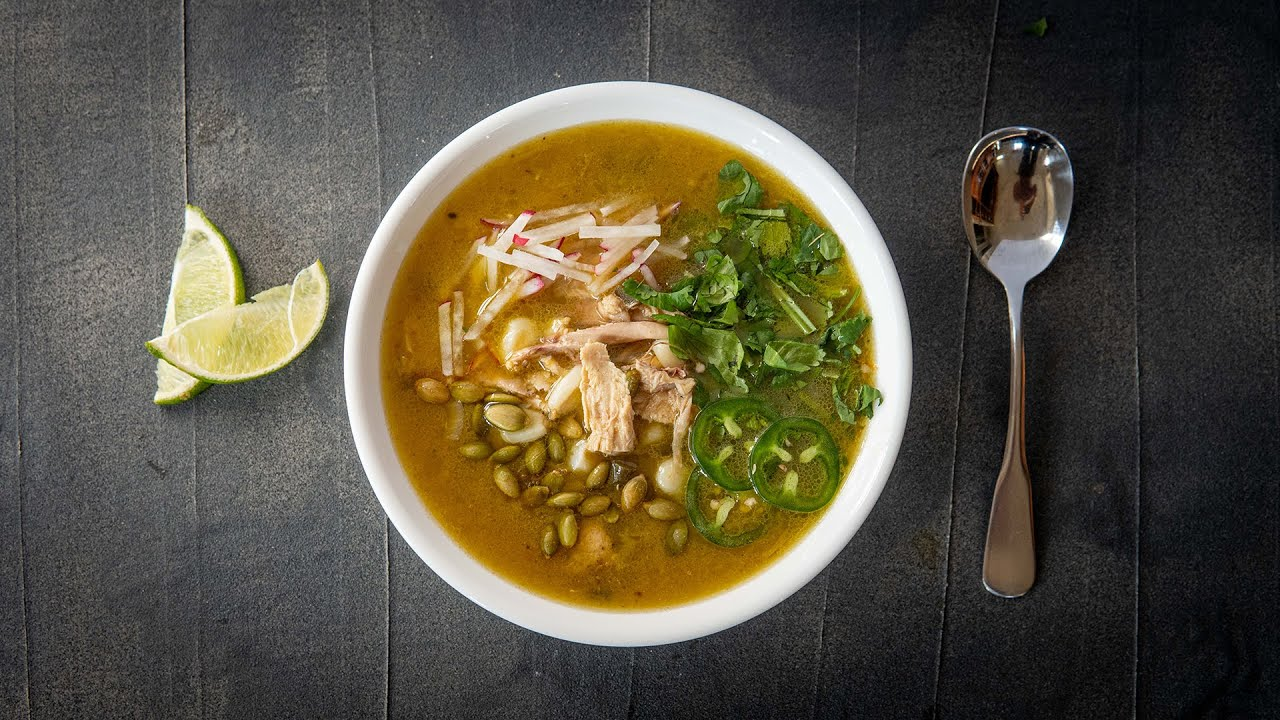
\includegraphics[width=1\textwidth,height=\textheight]{index_files/mediabag/cd0d3ee9e260eb552474.jpg}

\textbf{Prep Time:} NA \textbar{} \textbf{Cook Time:} NA \textbar{}
\textbf{Total Time:} 1 hr 30 min

\section{Ingredients}\label{ingredients}

\begin{itemize}
\tightlist
\item
  Tomatillos, 12-15
\item
  Poblano peppers, 3-4
\item
  Ghost pepper, 1
\item
  Serrano peppers, 2
\item
  Yellow onion, 1
\item
  Garlic, 6 cloves
\item
  Whole Chicken, 1
\item
  chicken stock, 1800 g
\item
  hominy, 850 g
\item
  Cumin, 3 g
\item
  Ground coriander, 2 g
\item
  Chili Powder, 2 g
\item
  Salt,
\item
  Black Pepper,
\item
  Pickled onions,
\item
  Jalapeños,
\item
  Crema,
\item
  Radishes, thinly sliced
\item
  Cilantro,
\item
  Cotija cheese,
\item
  Limes,
\item
  Pepitas,
\end{itemize}

\section{Instructions}\label{instructions}

\begin{enumerate}
\def\labelenumi{\arabic{enumi}.}
\tightlist
\item
  Turn the oven on broil at 500° F/260° C.
\end{enumerate}

Spread tomatillos, poblano and serrano peppers on a large tin foil
rimmed baking sheet. Broil for 5 minutes until blackened and charred.
Let cool 10 minutes.

Meanwhile, finely chop the yellow onion and garlic cloves. Add them to a
bowl.

Once cooled, finely chop the roasted tomatillos, poblanos, and serrano
peppers and add them to the bowl. 1. Cut the whole chicken into 10
pieces.

If you haven't broken down a chicken yet, check out the video for how I
do this.

Next, heat a thin layer of vegetable oil in a large Dutch oven over
medium-high heat.

Liberally season the chicken pieces with salt and pepper.

Add them to the Dutch oven to sear and brown on all sides. Set the
browned chicken pieces on a plate and turn the heat to medium-low. 1. To
the same pot that the chicken was browned in, add the bowl of chopped
vegetables, ground spices, and a pinch of salt to the pot. Sauté,
stirring occasionally, for 10-15 minutes.

Set the heat to low and sauté for another 15-20 minutes until everything
is caramelized and reduced. 1. Pour in the chicken stock and deglaze the
pot.

Add the browned chicken pieces. Bring the soup to a simmer and cook,
uncovered, for 20-30 minutes.

Remove the chicken pieces and shred them, picking out any bones or
inedible pieces. Return the shredded chicken to the soup and add the
hominy.

Taste it and add salt and pepper as needed. 1. Serve in bowls and top
with pickled red onion, sliced jalapeño, crema, radish, cilantro,
cotija, fresh squeezed lime, or any other desired toppings.



\end{document}
